\documentclass[11pt]{report}

\usepackage{amsmath}
\usepackage{amssymb}
\usepackage{amsfonts}
\usepackage{dsfont}
\usepackage{epsfig}
\usepackage{times}
\usepackage{multicol}
%\usepackage{mcode}

\usepackage{bm}

\usepackage{footnote}
\makesavenoteenv{tabular}

\usepackage{enumerate}
%\usepackage{enumitem}
\usepackage{pdfpages}
%\usepackage{hyperref}
\usepackage{calc}
\usepackage{verbatim}

\usepackage{geometry}
\geometry{margin=0.25in}

\usepackage{parskip}

\DeclareMathOperator{\Prob}{\mathbb{P}}
\DeclareMathOperator{\Exp}{\mathbb{E}}
\DeclareMathOperator{\Var}{\text{Var}}
\DeclareMathOperator*{\argmin}{\arg\min}
\DeclareMathOperator*{\argmax}{\arg\max}

\DeclareMathOperator{\SSS}{\mathcal{S}}

\newcommand{\ind}{{\mathds{1}}}

\newcommand{\bs}{\boldsymbol}

\newcommand{\be}{\begin{enumerate}}
\newcommand{\ee}{\end{enumerate}}

\newcommand{\teq}{\triangleq}
\newcommand{\tr}{{\text{\tiny T}}}

\newcommand*{\tbf}[1]{\ifmmode\mathbf{#1}\else\textbf{#1}\fi}
\newcommand{\E}{\mathbb{E}}
\newcommand{\R}{\mathbb{R}}
\renewcommand{\P}{\mathbb{P}}
\newcommand{\ep}{\varepsilon}


\newcommand{\abs}[1]{\left\lvert#1\right\rvert}

\begin{document}
\begin{center}
    {\bf\large APMA 1740/2610 2025: Homework 3}
\end{center}
%\noindent{\bf\Large BE SURE TO CHANGE TO THE APPROPRIATE HW NUMBER}
\medskip


\begin{enumerate}[1.]

    %%%%%%%%%%%%%%%%%%%%%%%%%%%%%%%%%%%%%%%%%%%%%%%




    \item {\bf Convergence in probability.} We say that a sequence of random variables $X_1,X_2,\dotsc$ converges in probability to another random variable $X$ if
          \[ \Prob\bigl(|X_n-X| > \epsilon\bigr) \to 0 \quad \text{as $n\to\infty$ for every $\epsilon > 0$}. \]
          It is often the case that $X$ is a deterministic constant, which is a trivial example of a random variable.

          Let $\theta\in\mathbb{R}$ and suppose that $\widehat\theta_n$ is an estimator of $\theta$.  Use Markov's inequality\footnote{Markov's inequality states that $\Prob\bigl(|Z| \geq \alpha\bigl) \leq \Exp(|Z|)/\alpha$ for every $\alpha > 0$.  Note that you can apply Markov's inequality to $|Y|^k$ by taking $Z=|Y|^k$.}  to prove the following: If the MSE of $\widehat\theta_n$ converges to zero (i.e., $\widehat\theta_n$ is consistent in MSE), then $\widehat\theta_n$ converges to $\theta$ in probability (i.e., $\widehat\theta_n$ is consistent in probability).

          This is a very useful fact because working with expectations (MSE) is often much easier than working with probabilities.

          %%%%%%%%%%%%%%%%%%%%%%%%%%%%%%%%%%%%%%%%%%%%%%%


          \color{blue}
          We want to show that
          \[\text{MSE}[\hat \theta_n] \to 0 \implies \P(\abs{\hat \theta_n - \theta} > \ep) \to 0\]

          Consider
          \begin{align*}
              \P(\abs{\hat\theta_n - \theta} > \ep) & = \P(\abs{\hat \theta_n - \theta} \geq \ep) - \P(\abs{\hat \theta_n - \theta} = \ep)        \\
                                                    & =  \P(\abs{\hat \theta_n - \theta} \geq \ep)  \qquad (\ep \to 0)                            \\
                                                    & = \P(\abs{\hat \theta_n - \theta}^2 \geq \ep^2)                                             \\
                                                    & \leq \frac{1}{\ep^2} \E[\abs{\hat \theta_n - \theta}^2] \qquad \text{(Markov's Inequality)} \\
                                                    & = \frac{1}{\ep^2} \text{MSE}[\hat \theta_n]
          \end{align*}

          By assumption, $\text{MSE}[\hat \theta_n] \to 0$ so $\P(\abs{\hat \theta_n - \theta} > \ep) \to 0$ as well.
          \color{black}


          \pagebreak

    \item {\bf Bias-variance tradeoff.} Consider the problem of flipping a coin $n$ times and then guessing the probability of heads. In other words, let $X_{1:n}$ be iid Bernoulli$(p)$ for $p\in[0,1]$ and let $\widehat p \teq \widehat p(X_{1:n})$ be an estimator of $p$.  Consider the following possible estimators $\widehat p$ of $p$:

          \begin{center}
              \begin{tabular}{ll}
                  $\displaystyle \vphantom{\frac{1}{1}} \widehat p_1 \teq 0.5$                                                   & This estimator ignores the data and always guesses 0.5.                 \\
                  $\displaystyle \vphantom{\frac{1}{1}} \widehat p_2 \teq  \bar X_n  \teq \textstyle n^{-1} \sum_{i=1}^n X_i$    & This estimator is simply the fraction of ones in the data.
                  %\footnote{This turns out to be the {\em maximum likelihood estimator} (MLE) for $p$. In an upcoming lecture we will take a more general look at MLEs.}  
                  \\
                  $\displaystyle \vphantom{\frac{1}{1}} \widehat p_3 \teq \frac{2}{n+2}\widehat p_1 + \frac{n}{n+2}\widehat p_2$ & This estimator moves $\bar X_n$ closer to $0.5$, more so for less data. \\
                  %		\footnote{This estimator can be viewed as the sample mean of $X_{1:n}$, along with an extra $0$ and an extra $1$, so that there are $n+2$ total data points. It turns out that this is a Bayesian estimator created by using the posterior mean of $p$ under a uniform prior. We will discuss Bayesian inference near the end of the semester, time permitting.} \\
              \end{tabular}
          \end{center}

          \begin{enumerate}
              \item Compute the bias, variance, and mean squared error (MSE) as functions of $n$ and $p$ for each of the three estimators.

                    \color{blue}
                    Bias:
                    \begin{align*}
                        \E[\hat p_1] - p & = \boxed{0.5 - p}                                                                                                                        \\
                        \E[\hat p_2] - p & = \E[\bar X_n] - p = \frac{1}{n} \sum_{i=1}^n \E[X_i] - p = p - p = \boxed{0}                                                            \\
                        \E[\hat p_3] - p & = \frac{2}{n+2} \E[\hat p_1] + \frac{n}{n+2} \E[\hat p_2] - p = \frac{2}{n+2} (0.5) + \frac{n}{n+2} (p) - p = \boxed{\frac{1 - 2p}{n+2}}
                    \end{align*}

                    Variance:
                    \begin{align*}
                        \Var[\hat p_1] & = \Var[0.5] = \boxed{0}                                                                                                                           \\
                        \Var[\hat p_2] & = \frac{1}{n^2} \sum_{i=1}^n \Var[X_i] = \frac{1}{n^2} \cdot n \cdot p(1-p) = \boxed{\frac{p(1-p)}{n}}                                            \\
                        \Var[\hat p_3] & = \frac{4}{(n+2)^2} \Var[\hat p_1] + \frac{n^2}{(n+2)^2} \Var[\hat p_2] =  \frac{n^2}{(n+2)^2} \frac{p(1-p)}{n} = \boxed{\frac{np(1-p)}{(n+2)^2}}
                    \end{align*}

                    Finally, since $\text{MSE}[\hat \theta] = \Var[\hat \theta] + b^2$,
                    \begin{align*}
                        \text{MSE}[\hat p_1] & = \boxed{(0.5 - p)^2}                                                                                  \\
                        \text{MSE}[\hat p_2] & = \boxed{\frac{p(1-p)}{n}}                                                                             \\
                        \text{MSE}[\hat p_3] & = \frac{np(1-p)}{(n+2)^2} + \left(\frac{1 - 2p}{n+2}\right)^2 = \frac{(4 - n)p^2 + (n-4)p +1}{(n+2)^2}
                    \end{align*}


                    \color{black}

              \item Which, if any, of these estimators is unbiased?  Which, if any, is consistent in probability? Why?

                    \color{blue}
                    $\hat p_2$ is unbiased since $\E[\hat p_2] = p$ for all $n$. Both $\hat p_2$ and $\hat p_3$ are consistent in probability since $\text{MSE}[\hat p_2] \to 0$ and $\text{MSE}[\hat p_3] \to 0$ and by Problem 1, consistence in MSE implies consistence in probability.
                    \color{black}

              \item For the case $n=5$, plot the three MSEs as a function of $p$ on the same graph.

                    \begin{center}
                        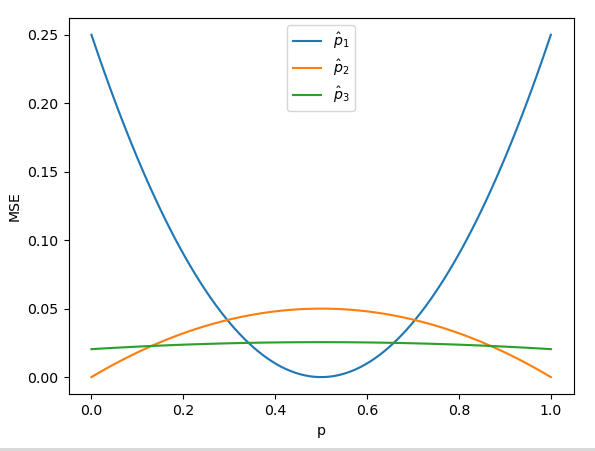
\includegraphics[width=0.8\textwidth]{Images/2c.png}
                    \end{center}

              \item For the case $n=5$, are any of the three estimators uniformly better than the others?  Why or why not?

                    \color{blue}
                    No. $\hat p_1$ optimizes for the case $p = 0.5$ while $\hat p_2$ optimizes for the case $p = 0$ or $p = 1$. $\hat p_3$ is a compromise between the two.
                    \color{black}

              \item For each of the three estimators, describe scenarios where that estimator is the one you would choose.  For example, suppose you have an a priori reason to believe that the coin is heavily weighted to almost always land on the same side.  Which estimator might you choose?

                    \color{blue}
                    If we strongly believed that the coin was fair, we would choose $\hat p_1$ as it has lowest MSE. If, however, we had reason to suspect the coin was heavily weighted towards one side, we would choose $\hat p_2$ which is unbiased and minimizes MSE at $p = 0$ and $p=1$. In other cases, it likely makes sense to use $\hat p_3$ as it is a compromise between the two.
                    \color{black}

          \end{enumerate}
          %%%%%%%%%%%%%%%%%%%%%%%%%%%%%%%%%%%%%%%%%%%%%%%




          \pagebreak

    \item {\color{blue} (Do not submit.)} {\bf Kernel density estimation.}
          Given an unknown density function $f$ on $\mathbb{R}$, and a sample $X_{1:n}\sim\ iid\ f$, our goal is to construct an estimator $\hat{f}_n(x;X_{1:n})$ of $f$. (And preferably one that has some kind of guarantee to approach $f$ as the sample size, $n$, goes to $\infty$.)

          Let $k$ (a ``kernel") be some density function $k(x)$ on $\mathbb{R}$, with the properties
          \[
              \int_{x=-\infty}^\infty x k(x) dx = 0\quad\text{(mean zero)} \qquad \& \qquad \int_{x=-\infty}^\infty x^2 k(x)dx = 1\quad\text{(standard deviation one)}
          \]
          Convince yourself that for any $w \in (0,\infty)$, $\displaystyle k_w(x) \triangleq \frac{1}{w}k(\frac{x}{w})$ is again a zero-mean density function, but now with standard deviation $w$ (sometimes called the ``bandwidth" of the kernel $k_w$).

          The ``kernel density estimator" of $f$, based on the kernel $k$ and the observations $X_{1:n}$, is
          \[
              \hat{f}_{n,w}(x;X_{1:n}) \triangleq \frac{1}{n} \sum_{k=1}^n k_w(x-X_k)
          \]
          In words, we center a density ($k_w$) at each sample point. The estimator at any location $x$ is just the average of the heights at $x$ of these $n$ centered densities. In this problem you will experiment with the results of using this method on a constructed (and hence known) density. The kernel will be the standard normal density, $\mathcal{N}(0,1)$, and hence
          \[
              k_w(x) = \frac{1}{w}\frac{1}{\sqrt{2\pi}} e^{-\frac{x^2}{2w^2}}
          \]

          The constructed density is
          \[ f(x) \teq \frac{1}{10}\sum_{\ell=1}^{10} \phi(x,\ell,\cos^2(\ell)) \]
          where $\phi(x,\mu,\sigma^2)$ is the pdf of a normal random variable with mean $\mu$ and variance $\sigma^2$.  This is called a mixture of Gaussians.\footnote{ Here is one way to create a sample of size $n$ from this distribution, say $X_1,\dotsc,X_n$.  First sample $n$ labels $L_1,\dotsc,L_n$ uniformly from the set $\{1,2,\dotsc,10\}$, for example, with {\tt L = randi(10,n,1)} in Matlab.  Now sample each $X_i$ independently according to Normal$(L_i,\cos^2(L_i))$, for example, with {\tt X = L + abs(cos(L)).*randn(n,1)} in Matlab.}
          \begin{enumerate}
              \item Plot $f$ over the interval $[-2,14]$ using bins of size $0.001$.  The function {\tt normpdf} can simplify your code in Matlab (but note that it takes $\sigma$, not $\sigma^2$, as an argument).  A worthwhile sanity check at this point is to generate a million samples from $f$ and make a histogram to verify that you get the same shape.
              \item
                    Generate a sample of size 200 from $f$.  Using the standard normal pdf as the kernel, compute kernel density estimates of $f$ for a variety of bandwidths.\footnote{Something like this might work in Matlab: {\tt x = -2:.001:14; fhat = zeros(size(x)); for k = 1:200, fhat = fhat + normpdf(x,X(k),w)/200; end}}  Graph three of these --- one with a (somewhat, but not excessively) too small bandwidth, one with a (somewhat, but not excessively) too large bandwidth, and one with a bandwidth that seems about right to you.  Put the true $f$ on the graphs, too, for comparison.  (Try to pretend that you don't know the real $f$, and think about which of these bandwidths you would choose.)
              \item Repeat part (b) 50 times (generate new data each time) using the same three bandwidths that you selected.  For each bandwidth, make a graph showing all 50 kernel density estimates and also the true density.\footnote{The matlab command {\tt hold on} is useful here.  Also, if you plot the true density last and use something like {\tt plot(x,f,'k','linewidth',2)} then it can be a lot easier to distinguish the true density from your 50 estimates.}  Interpret your plots in terms of bias and variance.  Which bandwidth do you think has the best mean integrated squared error (MISE)?
              \item Since you know the true $f$, you can (numerically) compute ISE. (You can't do this in a real problem, because $f$ is unknown.) For each of the three bandwidths used in part (c), compute the ISE for each of your 50 kernel density estimates from part (c) and average them to get an estimate of the MISE. Report your estimate of MISE for each bandwidth. Was your intuition from part (c) correct?
              \item
                    Repeat part (d) at a selection of bandwidths ranging from 0.01 to 3. (The more the better, but this can be computationally expensive.) Plot the curve of estimated MISE as a function of bandwidth. You should see a more-or-less smooth curve with an apparently unique minimum. (You will need higher resolution at smaller values of $w$. I used $w\in[0.01:0.01:0.3,\ .4:0.1:1,\  2,\  3]$, i.e. $w$ from 0.01 to 0.3 in steps of size 0.01; from 0.4 to 1 in steps of size 0.1; and $w = 2$
                    and $w=3$, for a total of 39 values. But this might take more time on your computer than you're willing to wait.)
          \end{enumerate}

          \pagebreak


    \item {\color{blue} (Do not submit.)} {\bf Cross validation for kernel density estimation.}
          \label{item:bandwidth}

          %This is a continuation of problem 3 of the previous HW, using the same target density and Gaussian kernel. Before proceeding, you should look at the HW 5 solutions and correct your mistakes, if any.

          In the previous problem, we explored the accuracy of various bandwidths with the luxury of knowing the target density. Of course we would not need to estimate the density in the first place if we it were already known. In this problem we will use the cross-validation approach developed in class to estimate a suitable bandwidth from the data.  Stone's theorem assures us that the resulting estimator of the density is asymptotically optimal, and hence we can expect good behavior for a large sample. How good is the approach at a modest sample size of $n=200$. (Modest, at least, in the context of nonparametric estimation.)

          Recall that cross validation selects the bandwidth using
          \[ \widehat h_n \teq \argmin_h \widehat J(h) \]
          where \[ \widehat J(h) \teq \int_{-\infty}^\infty \bigl(\widehat f_{n,h}(x)\bigr)^2 dx - \frac{2}{n}\sum_{i=1}^n \widehat f^{(i)}_{n-1,h}(X_i;{_i}X)  \]
          and $\widehat f^{(i)}_{n-1,h}(x_i;{_i}X)$
          is the kernel density estimator using all of the data except $X_i$.
          ({\em See below for a better way to write $\widehat J(h)$ when the kernel is the standard normal, and for some computational hints.})

          \begin{enumerate}[(a)]

              \item Select 200 independent samples from $f$. Compute $\widehat J(h)$ at each $h\in\{.01,.02,\ldots,.99,1\}$. Plot $\widehat J$.

              \item Choose the bandwidth, $\hat{h}^*$, that minimizes $\widehat J(h)$. Report the value of $\hat{h}^*$, and display both the density $f$
                    and the kernel density estimator that uses the cross-validated bandwidth. Put both functions on the same plot.

              \item Repeat (b) 50 times, and display all fifty estimators in one plot. Superimpose $f$, as was done in Problem 3. (Be sure to compute a new bandwidth each time.) Use the 50 estimators to compute the approximate MISE for cross-validated estimation of this $f$.

              \item How does cross validation compare to a fixed, hand-selected bandwidth? Was the MISE using cross-validation better than each of the fixed bandwidths from Problem 3(d)? What were the minimum and maximum bandwidths chosen by cross-validation for your 50 datasets?  Comment on your results.

          \end{enumerate}





          {\em Computational guidelines.}
          You can simplify $\widehat J(h)$ for the standard normal base kernel by noting that
          \begin{align*}
              \int \big(\widehat f_{n,h}(x)\big)^2 dx & = \int \Big(\frac{1}{n}\sum_{i=1}^n \kappa_h(x-X_i)\Big)^2 dx                                                                   \\
                                                      & = \frac{1}{n^2} \sum_{i=1}^n\sum_{j=1}^n \int \kappa_h(x-X_i)\kappa_h(x-X_j) dx                                                 \\
              \\ & = \frac{1}{n^2}\sum_{i=1}^n \sum_{j=1}^n \frac{1}{2\pi h^2} \int \exp\left(\frac{-(x-X_i)^2-(x-X_j)^2}{2h^2}\right) dx \\
                                                      & =  \frac{1}{n^2}\sum_{i=1}^n \sum_{j=1}^n \frac{1}{\sqrt{2\pi}(h\sqrt{2})} \exp\left(\frac{-(X_i-X_j)^2}{2(h\sqrt{2})^2}\right)
              = \frac{1}{n^2} \sum_{i=1}^n\sum_{j=1}^n \kappa_{h\sqrt{2}}(X_i-X_j)
          \end{align*}
          and
          \begin{align*}
              -\frac{2}{n} \sum_{i=1}^n \widehat f^{(i)}_{n-1,h}(X_i) & = -\frac{2}{n} \sum_{i=1}^n \frac{1}{n-1} \sum_{j\neq i} \kappa_h(X_i-X_j)                                   \\
                                                                      & = -\frac{2}{n(n-1)}\sum_{i=1}^n \left( \Big( \sum_{j=1}^n \kappa_h(X_i-X_j) \Big) - \kappa_h(X_i-X_i)\right) \\
                                                                      & = -\left(\frac{2}{n(n-1)} \sum_{i=1}^n \sum_{j=1}^n \kappa_h(X_i-X_j)\right) + \frac{2}{n-1}\kappa_h(0)      \\
                                                                      & = \frac{2\kappa_h(0)}{n-1}-\frac{1}{n^2} \sum_{i=1}^n \sum_{j=1}^n \frac{2n}{n-1}\kappa_h(X_i-X_j)
          \end{align*}
          so that
          \[ \widehat J(h) = \frac{2\kappa_h(0)}{n-1} + \frac{1}{n^2} \sum_{i=1}^n \sum_{j=1}^n \left( \kappa_{h\sqrt{2}}(X_i-X_j) - \frac{2n}{n-1}\kappa_h(X_i-X_j) \right)  , \]
          where $\kappa_h$ is the N$(0,h^2)$ pdf.
          Precompute the distances $X_i-X_j$ and store them in a $200\times 200$ matrix $D$.  Then in Matlab you need only use:
          \\ \\ {\tt sum(sum(normpdf(D,0,h*sqrt(2)) - 2*(n/(n-1))*normpdf(D,0,h)))}
          \\ \\ to get the double sum in the simplified expression for $\widehat J(h)$, which should evaluate very quickly.


          %%%%%%%%%%%%%%%%%%%%%%%%%%
          %			Problem  
          %%%%%%%%%%%%%%%%%%%%%%%%%%


          \pagebreak



    \item {\bf Estimating a pmf: consistency in mean square and in probability.} Let $\mathcal{I}$ be a discrete set (i.e., finite or countably infinite).  For convenience, we will label the elements with integers, i.e., $\mathcal{I}\teq\{1,2,\dotsc\}$.  Let $p\teq(p_1,p_2,\dotsc)$ be an unknown probability mass function (pmf) on $\mathcal{I}$, i.e., $0 \leq p_i \leq 1$ for all $i\in\mathcal{I}$ and $\sum_{i\in\mathcal{I}} p_i = 1$.  Suppose that $X_{1:n}$ is iid with common pmf $p$ over $\mathcal{I}$.
          \begin{enumerate}

              \item Find the maximum likelihood estimator (MLE) of $p$.  Call it $\hat p^{\text{\tiny MLE}}$. Note that $\hat p^{\text{\tiny MLE}}=(\hat p^{\text{\tiny MLE}}_1,\hat p^{\text{\tiny MLE}}_2,\dotsc)$ is a pmf and that it depends on both $n$ and the data $X_{1:n}$, which are suppressed in the notation.

                    \color{blue}
                    \begin{align*}
                        \hat p^{\text{MLE}} & = \argmax_{\tilde p} \tilde p(X_1 = x_1, X_2 = x_2, \ldots, X_n = x_n)                                  \\
                                            & = \argmax_{\tilde p} \prod_{j = 1}^n \tilde p(X_j = x_j)                                                \\
                                            & = \argmax_{\tilde p} \prod_{i \in \mathcal I} \tilde p_i^{\sum_{j=1}^{n} \ind\{X_j = i\} }              \\
                                            & = \argmax_{\tilde p} \sum_{i \in \mathcal I} \sum_{j=1}^{n} \ind\{X_j = i\} \log \tilde p_i             \\
                                            & =  \argmax_{\tilde p} \sum_{i \in \mathcal I} \frac{1}{n}\sum_{j=1}^{n} \ind\{X_j = i\} \log \tilde p_i \\
                                            & = \argmax_{\tilde p} \sum_{i \in \mathcal I} \hat p_i \log \tilde p_i                                   \\
                    \end{align*}

                    Now we can use Lagrange multipliers with $\sum_{i \in \mathcal I} \tilde p_i = 1$:
                    \[\frac{\partial}{\partial \tilde p_i} \left[\sum_{i \in \mathcal I} \hat p \log \tilde p_i + \lambda(1 - \sum_{i \in \mathcal I} \tilde p_i)\right] = \frac{\hat p_i}{\tilde p_i} - \lambda = 0 \implies \tilde p_i = \frac{\hat p_i}{\lambda}\]

                    But
                    \[\sum_{i \in \mathcal I} \tilde p_i = \sum_{i \in \mathcal I} \frac{\hat p_i}{\lambda} = 1 \implies \sum_{i \in \mathcal I} \hat p_i = \lambda\]
                    and since the empirical distribution is a pmf, $\lambda = 1$ which finally tells us
                    \[\hat p_i^{\text{MLE}} = \hat p_i = \frac{1}{n}\sum_{j=1}^{n} \ind\{X_j = i\}\]

                    \color{black}


              \item What is the MLE in this case? We have a name for it.

                    \color{blue}
                    The empirical distribution.
                    \color{black}

              \item For fixed $i$, compute the mean squared error (MSE) of $\hat p^{\text{\tiny MLE}}_i$. Call it $\text{MSE}_i$. Note that $\text{MSE}_i$ depends on $n$ and on the true pmf $p$, which are suppressed in the notation.

                    \color{blue}
                    \begin{align*}
                        \text{MSE}_i[\hat p] & = \Var[\hat p_i^{\text{MLE}}] + (\E[\hat p_i^{\text{MLE}}] - p_i)^2 \\
                                             & = \Var[\hat p_i] + \text{Bias}[hat p_i]^2                           \\
                    \end{align*}

                    First,
                    \begin{align*}
                        \text{Bias}[\hat p_i]   & = \E[\hat p_i] - p_i
                        = \frac{1}{n}\sum_{j=1}^n \E[\ind\{X_j = i\}] - p_i
                        = \frac{1}{n}\sum_{j=1}^n p_i - p_i
                        = p_i - p_i = 0                                \\
                        \text{Bias}^2[\hat p_i] & = 0
                    \end{align*}

                    And
                    \begin{align*}
                        \Var[\hat p_i] & = \Var\left[\frac{1}{n} \sum_{j=1}^{n} \ind\{X_j = i\} \right]               \\
                                       & = \frac{1}{n^2} \sum_{j=1}^n \Var[\ind\{X_j = i\}]                           \\
                                       & = \frac{1}{n^2} \sum_{j=1}^{n} \E[\ind\{X_j = i\}^2] - \E[\ind\{X_j = i\}]^2 \\
                                       & = \frac{1}{n^2} \sum_{j=1}^{n} p_i - p_i^2                                   \\
                                       & = \frac{1}{n}(p_i - p_i^2)
                        = \frac{p_i(1 - p_i)}{n}
                    \end{align*}

                    so
                    \[\text{MSE}_i[\hat p] = \frac{p_i(1 - p_i)}{n}\]
                    \color{black}

              \item For fixed $i$, show that $\hat p^{\text{\tiny MLE}}_i$ is consistent in mean square and in probability. Hint: Use part (c) and then Problem 1.

                    \color{blue}
                    Trivially,
                    \[\lim_{n \to \infty} \text{MSE}_i[\hat p] = \lim_{n \to \infty} \frac{p_i(1 - p_i)}{n} = 0\]
                    hence $\hat p_i^{\text{MLE}}$ is consistent in mean square.

                    By Problem 1, this also implies that $\hat p_i^{\text{MLE}}$ is consistent in probability.
                    \color{black}


              \item Define the total squared error of the whole pmf $\hat p^{\text{\tiny MLE}}$ to be
                    \[ \textstyle \sum_{i\in\mathcal{I}} (\hat p^{\text{\tiny MLE}}_i-p_i)^2 . \]
                    (This is similar to integrated squared error for pdfs, except that for pmfs we are using a sum, instead of an integral.) The total MSE is thus
                    \[ \textstyle \text{MSE} = \Exp\big(\sum_{i\in\mathcal{I}} (\widehat p_i^{\text{\tiny MLE}}-p_i)^2\big) .
                    \]
                    Show that
                    \[ \textstyle \text{MSE} = \sum_{i\in\mathcal{I}} \text{MSE}_i  , \]
                    and then use part (c) to show that
                    \[ \text{MSE} \leq \frac{1}{n} \]
                    regardless of the true pmf $p$.

                    \color{blue}
                    \begin{align*}
                        \text{MSE} & = \E\left[\sum_{i \in \mathcal I} (\hat p_i^{\text{MLE}} - p_i)^2\right]
                        = \sum_{i \in \mathcal I} \E[(\hat p_i^{\text{MLE}} - p_i)^2]                         \\
                                   & = \sum_{i \in \mathcal I} \text{MSE}_i
                        = \sum_{i \in \mathcal I} \frac{p_i(1 - p_i)}{n}
                        = \frac{1}{n} \sum_{i \in \mathcal I} p_i - p_i^2                                     \\
                                   & \leq \frac{1}{n} \sum_{i \in \mathcal I} p_i = \frac{1}{n}
                    \end{align*}
                    \color{black}


              \item Show that the whole pmf $\hat p^{\text{\tiny MLE}}$ is consistent for $p$ in mean square in the sense that $\text{MSE}\to 0$ as $n\to\infty$.

                    \color{blue}
                    By dominated convergence, since $\text{MSE} \leq \frac{1}{n}$ and $\frac{1}{n} \to 0$ as $n \to \infty$, $\text{MSE} \to 0$ as $n \to \infty$. Hence, $\hat p^{\text{MLE}}$ is consistent in mean square.
                    \color{black}

          \end{enumerate}



          %%%%%%%%%%%%%%%%%%%%%%%%%%
          %			Problem 
          %%%%%%%%%%%%%%%%%%%%%%%%%%

          \pagebreak



    \item {\bf MLE in exponential families.} A gamma$(\alpha,\beta)$ random variable has pdf
          \[ f_{\alpha,\beta}(x) = \frac{\beta^\alpha}{\Gamma(\alpha)}x^{\alpha-1}e^{-\beta x} \ind\{x > 0\} \]
          for parameters $\alpha,\beta > 0$.\footnote{Sometimes the gamma pdf is parameterized by $\alpha$ and $1/\beta$. If you are using software for gamma random variables, be sure you know which parameterization is being used.  (You don't need software in this problem.) $\Gamma(\alpha)\teq\int_0^\infty x^{\alpha-1} e^{-x} dx$ is the {\em gamma function}.} (In this problem, as usual, $\log=\log_e$.)
          \begin{enumerate}
              \item Express $f_{\alpha,\beta}$ as an exponential family and identify the sufficient statistics.

                    \color{blue}
                    Let
                    \begin{align*}
                        \lambda          & = (\alpha, \beta)                       \\
                        Z(\alpha, \beta) & = \frac{\Gamma(\alpha)}{\beta^{\alpha}} \\
                        h(x)             & = x^{-1}\ind\{x > 0\}                   \\
                        T(x)             & = (\log x, -x)
                    \end{align*}

                    Then,
                    \begin{align*}
                        \frac{1}{Z(\alpha, \beta)} h(x) e^{\lambda \cdot T(x)} & = \frac{\beta^\alpha}{\Gamma(\alpha)} x^{-1} \ind\{x > 0\} \exp\left(\alpha \log x - \beta x\right) \\
                                                                               & = \frac{\beta^\alpha}{\Gamma(\alpha)} x^{\alpha - 1} e^{-\beta x} \ind\{x > 0\}                     \\
                                                                               & = f_{\alpha, \beta}(x)
                    \end{align*}
                    so $f_{\alpha, \beta}$ is an exponential family with sufficient statistics $\log x$ and $-x$.
                    \color{black}

              \item Suppose that I collect this data set of size $5$:
                    \[ 1.45, \ 3.24, \ 1.07, \ 0.34, \ 2.29,  \]
                    and that I model it as iid gamma$(\alpha,\beta)$ for unknown parameters $\alpha,\beta$. It turns out that the MLE is\footnote{For the purposes of this problem, you can assume that this is the MLE to infinite numerical precision, although it is not really.}
                    \[ (\hat\alpha^\text{\tiny MLE},\hat\beta^\text{\tiny MLE})=(2.1955,1.3084) . \]
                    Compute the value of the following integral, using nothing more than about ten operations on a calculator (or, say, in the Matlab Command window).
                    \[ \int_0^\infty \log(x) \frac{1.3084^{2.1955}}{\Gamma(2.1955)}x^{2.1955-1}e^{-1.3084 x} dx . \]
                    (The point is that you are not supposed to use something like Mathematica to symbolically integrate this, or Matlab to numerically integrate it. Instead, you are supposed to use theory we developed in class.)

                    \color{blue}
                    \begin{align*}
                        \int_0^{\infty} \log x \frac{1.3084^{2.1955}}{\Gamma(2.1955)}x^{2.1955-1}e^{-1.3-84x}\; dx & = \int_0^{\infty} \log x \frac{(\hat \beta^{\text{MLE}})^{\hat \alpha^{\text{MLE}}}}{\Gamma(\hat \alpha^{\text{MLE}})} x^{\hat \alpha^{\text{MLE}}-1} e^{-\hat \beta^{\text{MLE}}x} \; dx \\
                                                                                                                   & = \int_0^{\infty} \log x f_{\hat \alpha^{\text{MLE}}, \hat \beta^{\text{MLE}}}(x)\; dx                                                                                                    \\
                                                                                                                   & = \E_f[\log X]                                                                                                                                                                            \\
                                                                                                                   & = \E_f[T_1(X)]                                                                                                                                                                            \\
                                                                                                                   & = \overline{T_1(X)}                                                                                                                                                                       \\
                                                                                                                   & = \frac{1}{5} \sum_{i=1}^5 T_1(x_i)                                                                                                                                                       \\
                                                                                                                   & = \frac{\log(1.45) + \log(3.24) + \log(1.07) + \log(0.34) + \log(2.29)}{5}                                                                                                                \\
                                                                                                                   & \approx 0.2729
                    \end{align*}
                    \color{black}
          \end{enumerate}


          \pagebreak

    \item[] \hspace{-3ex} {\bf For 2610 or for extra credit:}


          %%%%%%%%%%%%%%%%%%%%%%%%%%%%%%%%%%%%%%%%%%%%%%%





    \item {\bf Modes of convergence, a brief introduction.} There are many ways in which a sequence of random variables (say $W_1,W_2,\ldots$) can converge to another random variable (say $V$).
          These ``modes of convergence'' can be conveniently discussed in the context of  the special case in which $V=0$, by simply replacing $W_k$ with
          $W_k-V$ for each $k=1,2,\ldots$. Having made that simplification, consider these three particular modes of convergence:
          \begin{enumerate}[i.]
              \item $\displaystyle \Prob\left(\lim_{k\to\infty} W_k = 0\right) = 1$, ``almost sure convergence''
              \item $\displaystyle \lim_{k\to\infty}  \Prob\left(|W_k| > \epsilon\right) = 0, \text{for every $\epsilon>0$}$, ``convergence in probability''
              \item $\displaystyle \lim_{k\to\infty}  \Exp\left(|W_k|^2\right) = 0$, ``mean square convergence''
          \end{enumerate}
          What, if any, relationships exist between different modes of convergence? For most pairs, the relationships are qualified, e.g. mode `a' implies mode `b' if the $W_k$'s are uniformly bounded.
          Concerning the three modes listed above, there are two unqualified relationships: (1) almost sure convergence always implies convergence in probability, and (2) mean square convergence always implies convergence in probability. The first requires some elementary measure theory, and the second can be proven with the Markov inequality, as your saw in Problem 1.

          Oftentimes, the best way to understand the connections among the different modes is through specific counterexamples. Concerning the three modes defined here, there are six possible relationships (of the type `a' implies `b'). The unqualified relationships listed above address two of the six. None of remaining four are unqualified, and hence there are, in each case, counterexamples. Here we will construct a counterexample for each of the four.

          Let $X$ have the uniform distribution on $[0,1]$. Define a sequence of subsets of $[0,1]$, $A_1,A_2,\ldots \subseteq [0,1]$, as follows:
          \[
              \begin{array}{ccccccc}
                  A_1 = [0,1]                                                                                                                         \\
                  A_2 = [0,\frac{1}{2}] & A_3 = [\frac{1}{2},1]                                                                                       \\
                  A_4 = [0,\frac{1}{4}] & A_5 = [\frac{1}{4},\frac{2}{4}]
                                        & A_6 = [\frac{2}{4},\frac{3}{4}]    & A_7 = [\frac{3}{4},1]                                                  \\
                  A_8 = [0,\frac{1}{8}] & A_9 = [\frac{1}{8},\frac{2}{8}]
                                        & A_{10} = [\frac{2}{8},\frac{3}{8}] & A_{11} = [\frac{3}{8},\frac{4}{8}]
                                        & \cdots                             & A_{15} = [\frac{7}{8},1]                                               \\
                  \vdots                & \vdots                             & \vdots                             & \vdots & \vdots & \vdots & \cdots
              \end{array}
          \]
          For every $n=0,1,\ldots$ there are $2^n$ intervals of width $\frac{1}{2^n}$
          (namely $A_k$ for $k=2^n,\ldots,2^{n+1}-1$)
          which share endpoints but otherwise partition $[0,1]$.
          \begin{enumerate}[(a)]
              \item Define $\displaystyle W_k = \mathds{1}_{X\in A_k},\ k=1,2,\ldots$. Show that $W_k$ converges to zero in probability and mean square, but not almost surely.

                    \color{blue}
                    Assume $n = 2^k +j$ for some $j < 2^k$. Then we may write
                    \[W_n = \ind\{X \in A_n\} = \ind\{[\frac{j}{2^k}, \frac{j+1}{2^k}]\}\]

                    \tbf{Mean Square:}
                    \[\text{MSE}[W_n] = \E\abs{W_n}^2 = \E[\ind\{[\frac{j}{2^k}, \frac{j+1}{2^k}]\}^2] = \E[\ind\{[\frac{j}{2^k}, \frac{j+1}{2^k}]\}] = \P(X \in [\frac{j}{2^k}, \frac{j+1}{2^k}]) = \frac{1}{2^k} \to 0\]

                    \tbf{Probability:} By Problem 1, $MSE[W_n] \to 0\implies W_n \overset{\P}{\longrightarrow} 0$.

                    \tbf{Almost Sure:}
                    Suppose $\P(\lim_{n \to \infty} W_n = 0) = 1$. But $\forall x_0$, $\exists k$ such that $x_0 \in [\frac{j}{2^k}, \frac{j+1}{2^k}]$ (nested interval property). But then $W_n(x_0) = 1$ on a set with measure $2^{-k} > 0$. Contradiction.
                    \color{black}

              \item  Define $\displaystyle W_k = 2^k\mathds{1}_{X\in A_k},\ k=1,2,\ldots$. Show that $W_k$ converges to zero in probability but not in mean square and not almost surely.

                    \color{blue}
                    \tbf{Mean Square:}
                    \[\text{MSE}[W_n] = \E\abs{W_n}^2 = \E[2^{2n}\ind\{[\frac{j}{2^k}, \frac{j+1}{2^k}]\}] = 2^{2n}\P(X \in [\frac{j}{2^k}, \frac{j+1}{2^k}]) = 2^{2n-k} = 2^{2(2^{k} + j) - k} \not\to 0\]

                    \tbf{Probability:}
                    \[\P(\abs[W_n] > \ep) = \P(\abs{2^n \ind\{X \in A_n\}} > \ep) = \P(\ind\{[\frac{j}{2^k}, \frac{j+1}{2^k}]\} > \frac{\ep}{2^{n}}) = \P(X \in [\frac{j}{2^k}, \frac{j+1}{2^k}]) = \frac{1}{2^k} \to 0\]

                    \tbf{Almost Sure:}
                    \[\P(\lim_{n \to \infty} W_n = 0) = \P(\lim_{n \to \infty} 2^n \ind\{X \in A_n\} = 0) = \P(X \notin A_n \quad \forall n \geq N)\]
                    but by same argument as for (a), this is not possible.
                    \color{black}

              \item Find a sequence of intervals ($A_1,A_2,\ldots \subseteq [0,1]$), and a corresponding sequence of numbers ($\alpha_1,\alpha_2,\ldots$), such that if $\displaystyle W_k = \alpha_k\mathds{1}_{X\in A_k}$ for all $k=1,2,\ldots$, then $W_k$ converges to zero almost surely but not in mean square.

                    \color{blue}
                    Let $\alpha_k = \sqrt{2^k}$ and $A_k = [0, \frac{1}{2^{k}}]$ so $W_k = \sqrt{2^k} \ind\{X \in [0, \frac{1}{2^k}]\}$.

                    \tbf{Almost Sure:}
                    \[\P(\lim_{k \to \infty} W_k =0) = \P(\lim_{k \to \infty} \sqrt{2^k} \ind\{X \in [0, \frac{1}{2^k}]\} = 0) = \P(X \notin \lim_{k \to \infty} [0, \frac{1}{2^k}]) = 1 - \lim_{k \to \infy} \frac{1}{2^k} = 1 - 0 = 1\]

                    \tbf{Mean Square:}
                    \[\lim_{k\to \infty} \E\left[\abs{ \sqrt{2^k} \ind\{X \in [0, \frac{1}{2^k}]\}}^2\right] = \lim_{k \to \infty} 2^k\cdot \P(X \in [0, \frac{1}{2^k}]) = \lim_{k \to \infty} 2^k \cdot \frac{1}{2^k} = 1 \neq 0\]
                    \color{black}

          \end{enumerate}


          %%%%%%%%%%%%%%%%%%%%%%%%%%%%%%%%%%%%%%%%%%%%%%%



          \pagebreak


    \item {\bf Box-car kernel: pointwise consitency.}
          Consider the box-car kernel $\kappa(x) \teq \ind\{|x|\leq 1/2\}$ and define the family of box-car kernels in the usual way via $\kappa_h(x)\teq \kappa(x/h)/h$, where $h > 0$ is the bandwidth. (In the lecture I assumed that the standard deviation of the kernel was one, but this was only for convenience.)
          Let $X_{1:n}$ be iid with pdf $f$ and corresponding cdf $F$, and let $\widehat f_{n,h}$ be the kernel density estimator of $f$ using $\kappa_h$.
          \begin{enumerate}
              \item Fix $x$. Show that
                    \[ \Exp\bigl(\widehat f_{n,h}(x)\bigr) = \frac{F(x+h/2)-F(x-h/2)}{h} \]
                    and that
                    \[ \Var\bigl(\widehat f_{n,h}(x)\bigr) = \frac{F(x+h/2)-F(x-h/2) - \bigl(F(x+h/2)-F(x-h/2)\bigr)^2}{nh^2} . \]
                    Hint: $\widehat f_{n,h}(x)$ is the average of iid Bernoulli random variables.

                    \color{blue}
                    \begin{align*}
                        \hat f_{n, h}(x)       & = \frac{1}{n} \sum_{i=1}^n \kappa_h(x - X_i)                                                                                                        \\
                                               & = \frac{1}{nh} \sum_{i=1}^n \kappa(\frac{x - X_i}{h})                                                                                               \\
                        \E[\hat f_{n, h}(x)]   & = \E\left[\frac{1}{nh} \sum_{i=1}^n \ind\left\{\abs{x - X_i} \leq \frac{h}{2}\right\}\right]                                                        \\
                                               & = \frac{1}{nh} \sum_{i=1}^{n} \E\left[\ind\{\abs{x - X_i} \leq \frac{h}{2}\} \right]                                                                \\
                                               & = \frac{1}{nh} \sum_{i=1}^{n} \P(\abs{x - X_i} \leq \frac{h}{2})                                                                                    \\
                                               & = \frac{1}{nh} \sum_{i=1}^{n} \P(\abs{X_i} \leq x + \frac{h}{2})                                                                                    \\
                                               & = \frac{F(x + \frac{h}{2})  - F(x - \frac{h}{2})}{h}                                                                                                \\
                        \Var[\hat f_{n, h}(x)] & = \Var\left[\frac{1}{nh} \sum_{i=1}^n \ind\left\{\abs{x - X_i} \leq \frac{h}{2}\right\}\right]                                                      \\
                                               & = \frac{1}{n^2h^2} \sum_{i=1}^{n} \Var\left[\ind\{\abs{x - X_i} \leq \frac{h}{2}\} \right]                                                          \\
                                               & = \frac{1}{n^2h^2} \sum_{i=1}^{n} \E\left[\ind\{\abs{x - X_i} \leq \frac{h}{2}\}^2\right] - \E\left[\ind\{\abs{x - X_i} \leq \frac{h}{2}\}\right]^2 \\
                                               & = \frac{1}{n^2h^2} \sum_{i=1}^{n} \P(\abs{X_i} \leq x + \frac{h}{2}) + \P(\abs{X_i} \leq x + \frac{h}{2})^2                                         \\
                                               & = \frac{F(x + \frac{h}{2}) - F(x - \frac{h}{2}) + (F(x + \frac{h}{2}) - F(x - \frac{h}{2}))^2}{nh^2}
                    \end{align*}
                    \color{black}

              \item Fix an $x$ for which $f$ is continuous at $x$.  Show that if $h_n\to 0$ and $nh_n\to\infty$ as $n\to\infty$, then $\widehat f_{n,h_n}(x)$ is consistent for $f(x)$ in probability.

                    \color{blue}
                    By problem 1, it suffices to show that $\hat f_{n, h}(x)$ is consistent in MSE:
                    \[\text{MSE}[\hat f_{n, h_n}]  = \Var[\hat f_{n, h_n}] + (\E[\hat f_{n, h_n}] - f)^2\]

                    First, we calculate the bias:
                    \[\E[\hat f_{n, h_n}] - f = \frac{F(x + \frac{h_n}{2}) - F(x - \frac{h_n}{2})}{h_n} - f(x) \overset{h_n \to 0}{\longrightarrow} F'(x) - f(x) = f(x) - f(x) = 0 \]

                    Then
                    \begin{align*}
                        \Var[\hat f_{n, h_n}] & = \frac{F(x + \frac{h_n}{2}) - F(x - \frac{h_n}{2}) + (F(x + \frac{h_n}{2}) - F(x - \frac{h_n}{2}))^2}{nh_n^2} \\
                                              & \overset{h_n \to 0}{\longrightarrow} \frac{f(x)}{nh_n} + \frac{f^2(x)}{n}                                      \\
                                              & \overset{n \to \infty}{\longrightarrow} 0
                    \end{align*}

                    \color{black}

          \end{enumerate}

          \pagebreak


    \item {\bf Estimating a pmf: strong consistency.} This is a continuation of Problem 5:
          \begin{enumerate}
              \item For fixed $i$, use the strong law of large numbers to show that $\hat p^{\text{\tiny MLE}}_i$ is strongly consistent for $p_i$, meaning $\hat p^{\text{\tiny MLE}}_i\to p_i$ almost surely as $n\to\infty$.

                    \color{blue}
                    From Problem 5, $\hat p_i^{\text{MLE}} = \frac{1}{n}\sum_{j=1}^{n} \ind\{X_j = i\}$.

                    Let $Y_j = \ind\{X_j = i\} \sim \text{Bernoulli}(p_i)$ for $j=1:n$.

                    By the Strong Law of Large numbers,
                    \[\frac{1}{n}\sum_{j=1}^{n} \ind\{X_j = i\} = \bar Y \overset{a.s.}{\longrightarrow} \E[Y_i] = p_i\]
                    so, in particular,
                    \[\hat p_i^{\text{MLE}} \overset{a.s.}{\longrightarrow} p_i\]

                    \color{black}


              \item For a pmf $q$ and a set $B\subseteq \mathcal{I}$ we define $q(B)\teq \sum_{i\in B}q_i$ to be the probability that the pmf assigns to the set $B$. For a fixed set $B$, show that $\hat p^{\text{\tiny MLE}}(B)$ is strongly consistent for $p(B)$ as $n\to\infty$.

                    \color{blue}
                    \begin{align*}
                        \hat p^{\text{MLE}}(B) & = \sum_{i \in B} \hat p_i^{\text{MLE}}                                        \\
                                               & = \sum_{i \in B} \frac{1}{n}\sum_{j=1}^{n} \ind\{X_j = i\}                    \\
                                               & = \frac{1}{n}\sum_{j=1}^{n} \sum_{i \in B} \ind\{X_j = i\}                    \\
                                               & \overset{a.s.}{\longrightarrow} \E\left[\sum_{i \in B} \ind\{X_j = i\}\right] \\
                                               & = \sum_{i \in B} \E[\ind\{X_j = i\}]                                          \\
                                               & = \sum_{i \in B} p_i = p(B)
                    \end{align*}
                    \color{black}


              \item Show that $\hat p^{\text{\tiny MLE}}$ is strongly consistent for $p$ in total variation distance, meaning that
                    \[ \textstyle \text{\sc tv}(\hat p^{\text{\tiny MLE}},p) \teq \sup_{B\subseteq\mathcal{I}} |\hat p^{\text{\tiny MLE}}(B)-p(B)| \to 0 \]
                    almost surely as $n\to\infty$.

                    \color{blue}
                    \begin{align*}
                        \text{TV}(\hat p^{\text{MLE}}, p) & = \sup_{B \subseteq \mathcal I} \abs{\hat p^{\text{MLE}}(B) - p(B)}            \\
                                                          & \overset{a.s.}{\longrightarrow} \sup_{B \subseteq \mathcal I} \abs{p(B)- p(B)} \\
                                                          & = \sup_{B \subseteq \mathcal I} 0 = 0
                    \end{align*}
                    \color{black}
          \end{enumerate}






          %%%%%%%%%%%%%%%%%%%%%%%%%%
          %			Problem 
          %%%%%%%%%%%%%%%%%%%%%%%%%%


          \pagebreak


    \item {\bf Another kind of cross validation and an introduction to order statistics.}
          Cross validation is a general approach to assessing the performance of an estimator without the necessity of collecting additional ``out-of-sample" data.
          An example is the leave-one-out method for
          choosing a smoothing parameter, such as the bandwidth $h$ in kernel density estimation.
          The idea is to ignore one of the samples, form the estimator from the remaining samples,
          and evaluate performance based on the unused sample. This can be
          repeated for every observation, and the results can be pooled.

          If, for example, we are looking for a good bandwidth $h$, then the entire process can be repeated for each of a selection of bandwidths,
          and the empirically best bandwidth chosen.
          (Variations include the leave-$k$-out method, in which each evaluation is based on $k>1$ samples that were removed in forming the estimator.)

          This can work very well or very poorly. The MISE approach explored in previous problems (and supported by Stone's theorem) often works very well.
          Here we will look at a similar approach using likelihoods that often works very poorly.

          Start with the $n$ leave-one-out estimators for $f$ used in Problem \ref{item:bandwidth}:
          \[
              \left\{\hat{f}^{(i)}_{h}(x;{_i}X)\right\}_{i=1:n} \quad \text{where}\quad
              \hat{f}^{(i)}_{h}(x;{_i}X) = \frac{1}{n-1}\sum_{\substack{ k=1:n\\ k \neq i}} \kappa_h(x-X_k)
          \]
          (For convenience, we will write $\hat{f}^{(i)}_{h}(x;{_i}X)$, and occasionally just $\hat{f}^{(i)}$, instead of $\hat{f}^{(i)}_{n-1,h}(x;{_i}X)$.)
          In problem \ref{item:bandwidth}, $\hat{f}^{(i)}$ is used to make an estimate of the ISE for a given value of $h$.

          A compelling alternative is to use $\hat{f}^{(i)}$, instead, to estimate the likelihood:
          $$
              \tilde{J}(h)=\prod_{l=1}^n \hat{f}^{(i)}_h(X_i;{_i}X)
          $$
          and then search for $h$ to {\em maximize} $\tilde{J}(h)$. After all, in many typical scenarios the maximum likelihood estimator has a number of excellent properties, and $\tilde{J}$ would appear to be a sensible substitute.

          In this problem, we will assume that the true (but unknown) density is the exponential density with parameter one: $f(x)=e^{-x}$ on $x \geq 0$. The estimator is
          \[
              \hat{f}_h(x;X_{1:n})=\frac{1}{n}\sum_{k=1}^n \kappa_h(x-X_k)
          \]
          where $\kappa$ is
          the box-car kernel used in the previous homework, $\kappa(x) = \ind_{|x|\leq 1/2}$, and hence
          $\kappa_h(x)=\frac{1}{h}\ind_{|x|\leq h/2}$.

          For each $n$, let $h_n^* = \text{argmax} \tilde{J}(h)$. The problem is to show that $\hat{f}_{h_n^*}$ {\em cannot} be a consistent estimator for $f$.

          Here is one way to do this:
          \begin{enumerate}

              \item Let $X_{(1)}<X_{(2)}<\cdots<X_{(n)}$ be the {\em order statistics}
                    of $X_1,\ldots,X_n$, so that $\displaystyle X_{(1)}=\min_k X_k$,
                    $\displaystyle X_{(2)}=\min_{k:X_k>X_{(1)}} X_k$,
                    $\displaystyle X_{(3)}=\min_{k:X_k>X_{(2)}} X_k$,
                    and so on, up to
                    $\displaystyle X_{(n)}=\min_{k:X_k>X_{(n-1)}} X_k$ $=$
                    $\displaystyle \max_k X_k$.
                    Derive the joint density of the $n$ order statistics:
                    $$
                        f_{X_{(1)},\ldots,X_{(n)}}(x_1,\ldots,x_n)=
                        \left\{
                        \begin{array}{ll}
                            n! \prod_{k=1}^n e^{-x_k} & \mbox{if $x_1<x_2<\ldots <x_n$} \\
                            0                         & \mbox{otherwise}
                        \end{array}
                        \right.
                    $$

              \item
                    Change variables: Let $Y_{(i)}=X_{(i)}$ for $i=1,\ldots,n-1$ and
                    $Y_{(n)}=X_{(n)}-X_{(n-1)}$, and
                    compute the joint density of $Y_{(1)},Y_{(2)},\ldots,Y_{(n)}$.\footnote{The change-of-variables formula for densities is the same one you use for integrals (and for the same reasons): If the random vector $\vec{X}\in\mathbb{R}^n$ has density
                        $\alpha(\vec{x})$, and if $\vec{Y} = m(\vec{X})$ for some smooth and one-to-one function $m:\mathbb{R}^n\to\mathbb{R}^n$, with smooth inverse
                        $m^{-1}$, then $\vec{Y}$ has density
                        \[
                            \beta(\vec{y}) = \alpha(m^{-1}(\vec{y})) \left|\frac{\partial x_{1:n}}{\partial y_{1:n}} \right|
                        \]
                        where $ \left|\frac{\partial x_{1:n}}{\partial y_{1:n}} \right|$ is the determinant of the Jacobian.
                    }


              \item Compute the marginal density on $Y_{(n)}$.

              \item Show that
                    $$
                        h^*_n = \text{argmax}_h \prod_{i=1}^n \hat{f}^{(i)}_h(X_i;{_i}X)
                    $$
                    does not converge to zero. (Hint: show that $\displaystyle  \text{argmax}_h \prod_{i=1}^n \hat{f}^{(i)}_h(X_i;{_i}X) = 0$ whenever $h<2Y_{(n)}$.)

          \end{enumerate}

          In this formulation of cross validation, consistency requires a delicate balance between the tails of the kernel and the tails of the (unknown) density $f$. Basically, the tails of $f$ cannot be ``too heavy" relative to the tails of $\kappa$.






\end{enumerate}

\end{document}